




\section{Discussion}
(Comment on your results, explain what those results mean, interpret the results in a wider context. Also indicate which results were expected or unexpected, and provide an explanation for the unexpected results)

\subsection{Special cases where door heights are really close to each other or when room elevation heights are close to each other}

\subsection{Bad door matching in building 127 elev 0.31}

\subsection{Not removing a interrupting wall of RAC building}

\subsection{Removing walls to the outside}

\subsection{When to use minimum elevation or clippingheight}


\subsection{When to translate the data and when not to}

\subsection{A problem Where the translation of the doors will happen on one floor but not on the other due to the way that it checks for values.}

\subsection{narrow corriodors can block of the rest of the building with regards to nodes}

\subsection{Use for general IFC data}
- You can use the ifc open shell for general ifc data

\subsection{Problems with the data}
- Elevation not matching
- Walls where there shouldn't be walls


\subsection{Optimal node placement}
- Talk about different approaches to doing optimal node placement

\section{Conclusion}

\section{Future work}\label{Future_work}
\subsection{Walking up stairs}
The Spot robot has the ability to walk up and down stairs. A natural progression of this project is therefore to program Spot to walk up or down stairs to different floors. This way Spot can traverse around different floors of the building.

\subsection{Using a more complex algorithm for placing room nodes}
Another focus area for further development of this project is to develop a better method for placing the room nodes. At the moment the room nodes are placed using the K-means algorithm which is not an optimal placement strategy. Experimenting with different placement strategies and analysing the amount of coverage given for each is an interesting problem for further work.

\subsection{Taking into consideration the battery time for the robot when} developing the route
Furthermore to take into consideration the battery time of the robot when developing the route is also an area worth looking at for future work. In this project it is assumed that the battery time of the robot is sufficient for it to traverse one entire floor plan, but this assumption has not been put under scrutiny. It could be interesting to do some analysis of battery time compared with the route traversed. Finding the optimal path around the building and taking into consideration the battery capacity of Spot becomes especially when wanting for it to traverse multiple floor plans.

In further works of the project the program could have a recursive structure checking if the robot can actually traverse the floor plan and then prioritising which rooms it should traverse if not.


\subsection{Doing the actual programming of the robot}
This is part one of a 2 part project series where the second part of the project will be actually programming Spot to traverse the path generated in this part of the project.




\begin{comment}
\subsection{Grid vs graph connectivity}
Explain
\begin{itemize}
    \item both methods 
    \item that the graph doesn't work on weird buildings but grid system does.
    \item That grid scales badly with building size but graph doesn't
    \item f
    \item f
    \item f
    \item Maybe variation in node sizes help
    \item That the robot needs a certain node size to work properly. It doesn't work on nodes in the $mm^2$ range.
\end{itemize}


To make the robot walk from one room to another or one place in the building to another, it is important to understand the and decide on a way to implement the connectivity between the rooms. There are mainly two different kinds of implementations; a graph connectivity implementation and a grid implementation.
\\\\
The grid implementation works by discretizing the floor of the building into a grid with nodes of a specific size; the smaller the node size the higher the resolution of the grid.
\\
The graph connectivity approach works by representing each room/area by a node/dot which will be connected by a line to other rooms in the floor.

The different implementations have different advantages and limitations. For example computationally the graph connectivity approach is much more scalable with bigger buildings or construction sites where as implementing a grid system in these situations will be more taxing computationally since a lot of nodes will have to be calculated. 

On the other hand the advantage of the grid method is that its pathfinding algorithms will work on all building shapes. 
Imagine the floor plan of the building below:


\begin{figure}[H]
    \centering
    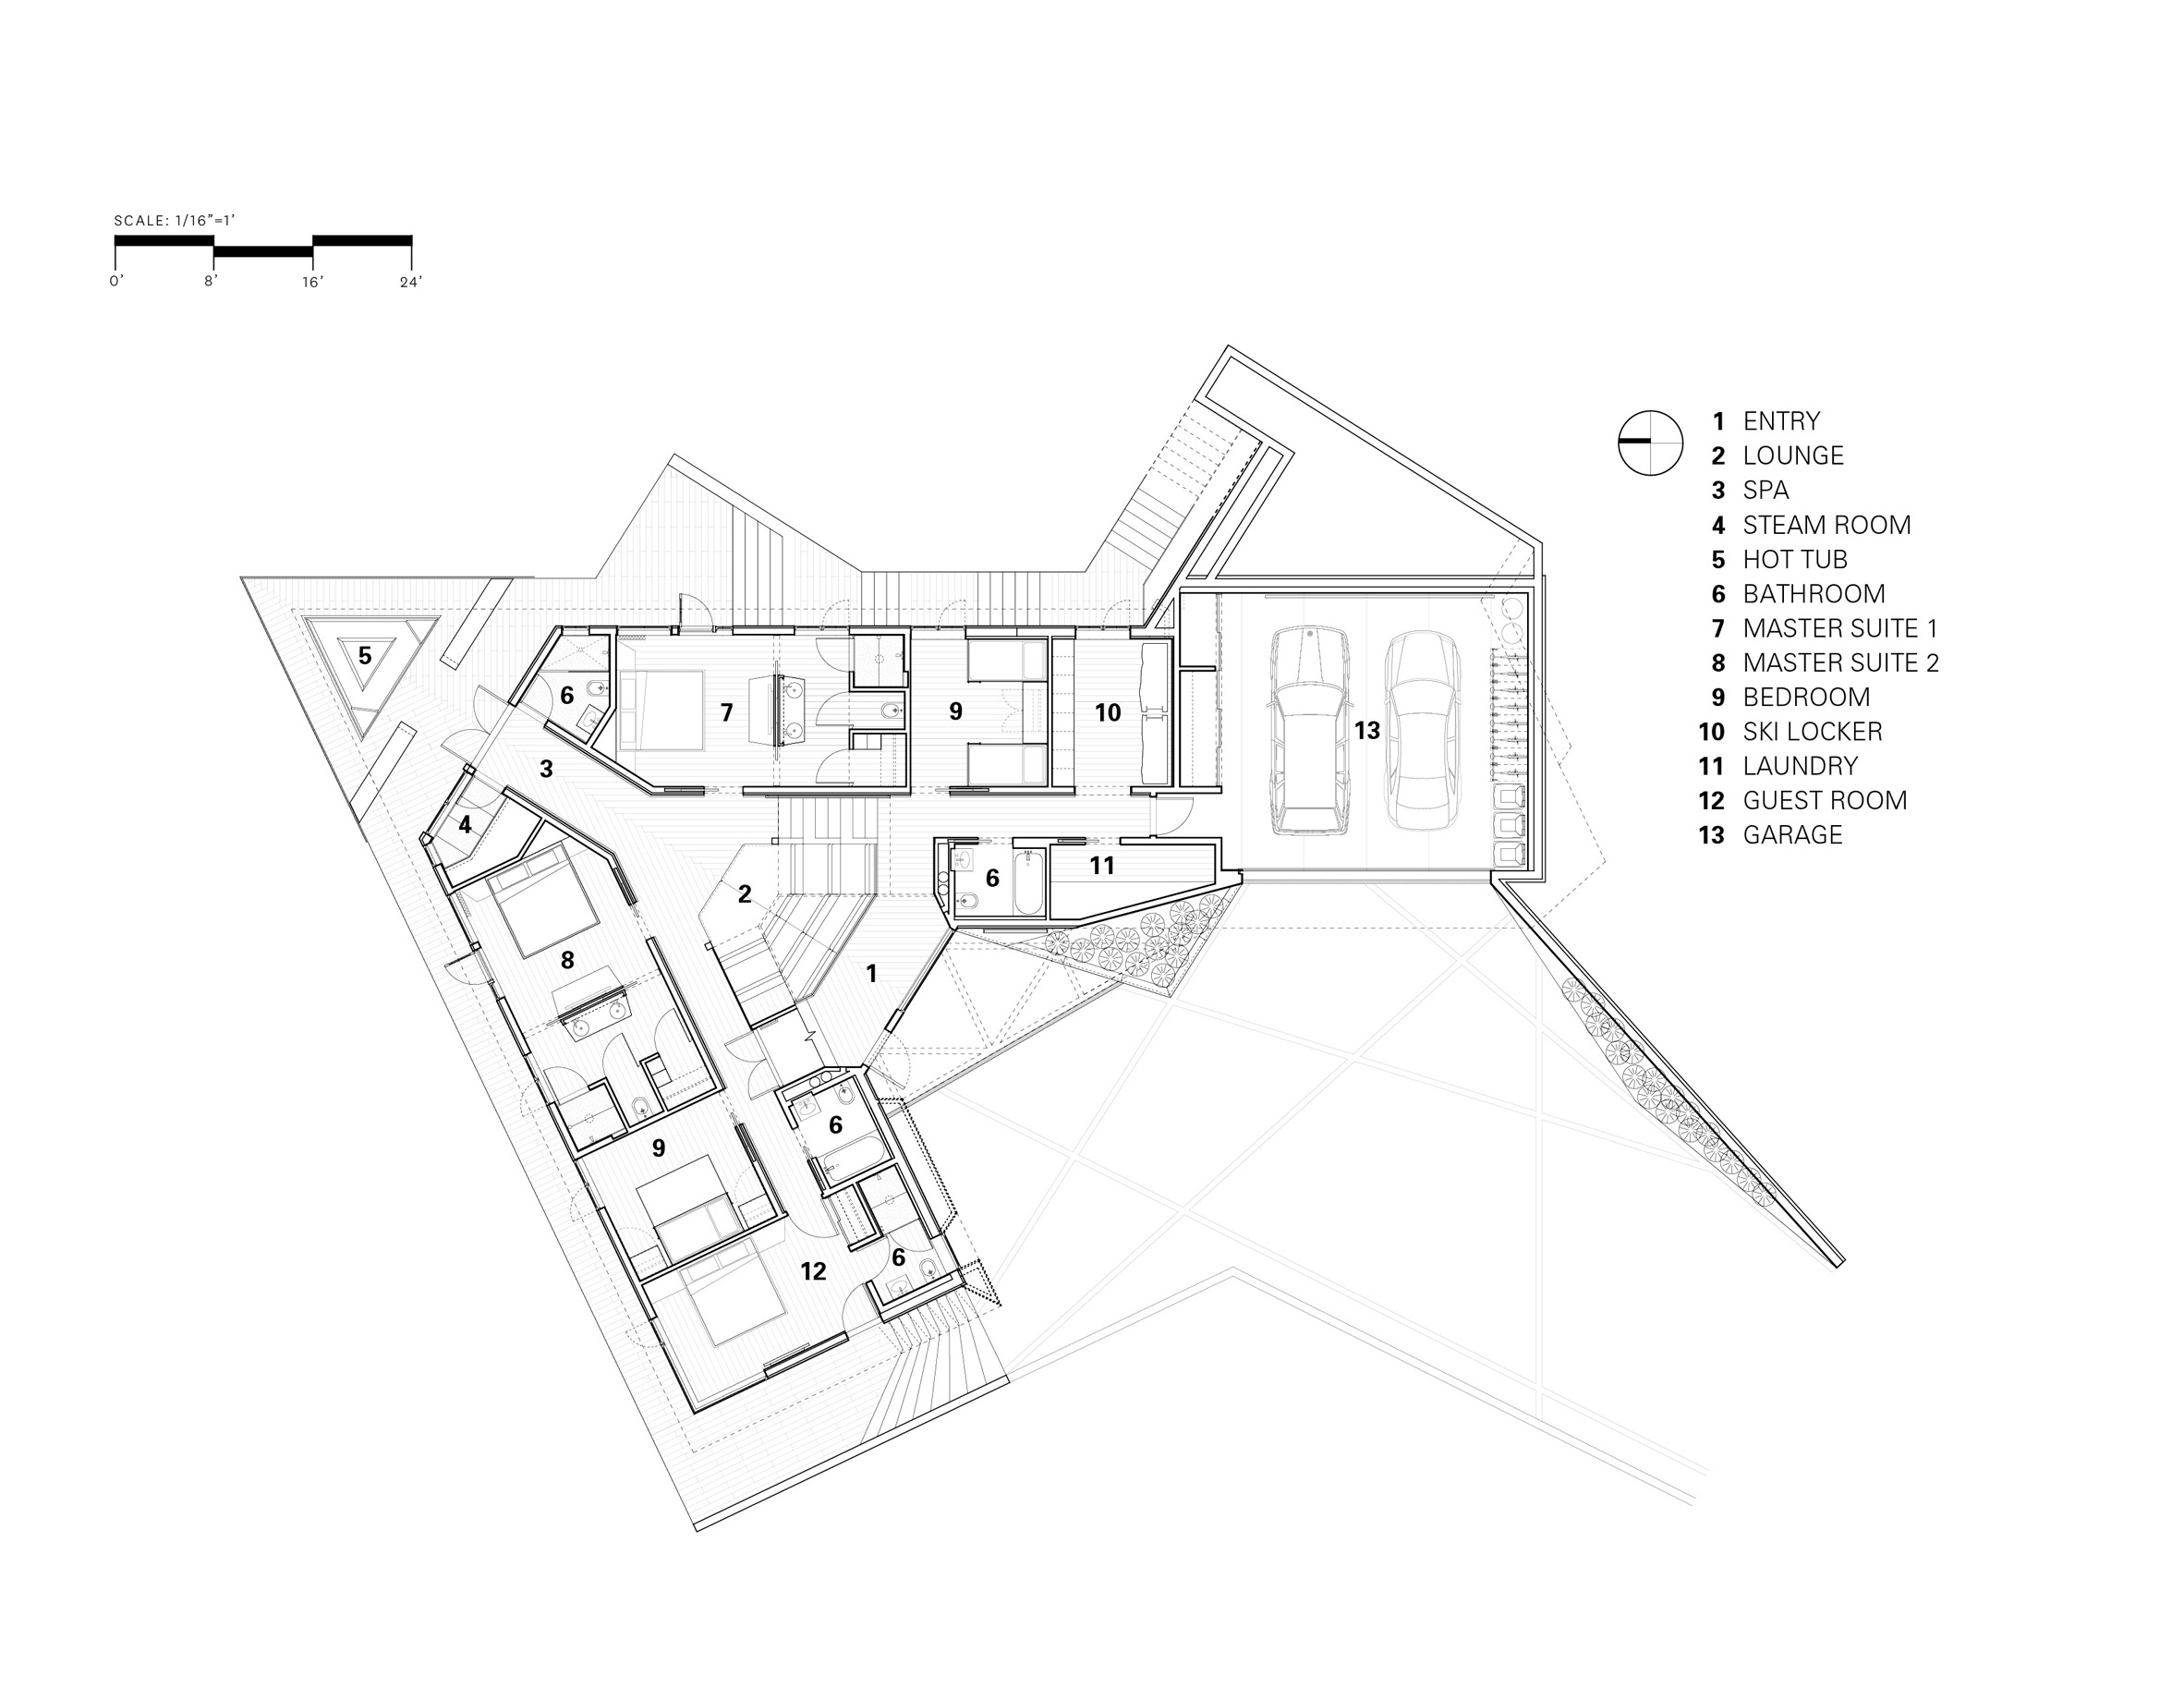
\includegraphics[width=1\textwidth]{fig/weird_floorplan.png}
    \label{}
    \caption[Weird floor plan]{Weird floor plan~\cite{weird_building}}
\end{figure}

When using a grid system apporach it will be possible to get an agent to walk from area 12 to 13 by specifically telling it which nodes are walkable and which nodes are not e.g walls. This will not be possible for the graph connectivity graph. The graph will here see only that area 12 and 13 are connected but not in which way. The method will draw a straight line between the two points and not see that the areas in reality are connected by the long pathway that goes through the entire floor plan.


\subsection{Grid system paper}
In this paper \cite{xu2017bim} they have the goal of solving “Accurate and efficient indoor path planning” in BIM models. The way they have implemented it is by using the grid system. 

\begin{figure}[H]
    \centering
    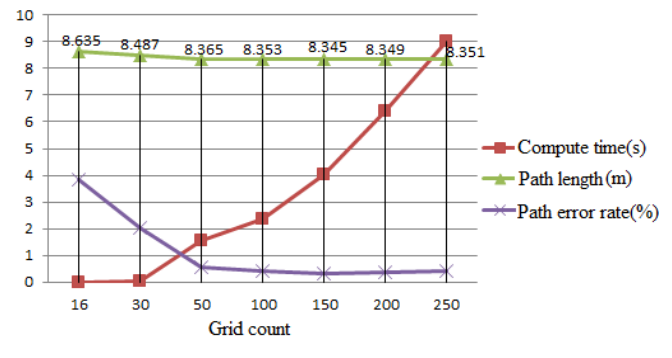
\includegraphics[width=1\textwidth]{fig/graph_grid_system.PNG}
    \caption{Graph showing computation cost as a function of grid count~\cite{xu2017bim}}
    \label{}
\end{figure}

They show what happens with the computation time when increasing the number of nodes. And also shows how minimal an effect it has on the path length.

Skriv om Convex decomposition vs alternativer(K means)

\\\\
\subsection{Conclusion}
blabal


\subsection{Future work}
You can write about slam
Write about stairs
Write about the whole thing about actually getting the robot to traverse the route and programming the robot
\end{comment}